\chapter{Implementation}

In the this chapter, we delve into practical exploration of the t-SimCNE framework, a novel method designed to enable unsupervised visualization of image datasets via contrastive learning. During implementatioin we relied on the code from the t-SimCNE GitHub repository, which provided the foundational codebase for this study.

\section{Training Settings}

Following the steps of Böhm et al. (2023) \cite{tsimcne}, we reproduced the training environment and model's settings in a similar way.

\subsection{Model Architecture}

The model utilizes a ResNet architecture, specifically a ResNet18. After feature extraction through the ResNet backbone, the model employs a fully-connected projection head.

\subsection{Pre-training}
The model is first pre-trained to output 128-dimensional embeddings for 100 epochs. This stage uses the full architecture, including the backbone and the projection head, to stabilize the feature space before reducing dimensionality.

\subsection{Fine-tuning}
After pre-training, the model undergoes a fine-tuning process where only the 2D readout layer is initially fine-tuned for 10 epochs to adjust to the lower-dimensional output. Subsequently, the entire network is fine-tuned for an additional 40 epochs to refine the 2D embeddings.

\subsection{Optimizer}
Stochastic Gradient Descent (SGD) with momentum (set to 0.9) is used. This optimizer is effective for navigating the complex landscapes of high-dimensional data typical of deep learning tasks.

\subsection{Learning Rate}
The initial learning rate is set to 0.12, scaled by the batch size relative to 256. This learning rate warm-ups over the first ten epochs, after which it follows a cosine annealing schedule down to zero. 

\subsection{Data Augmentation}
Essential to the contrastive learning approach, data augmentations such as random cropping and flipping are applied to generate diverse views of the same image, enhancing the model's ability to generalize from unlabelled data.

\section{Reproducing results}

My implementation began with the CIFAR-10 dataset, a standard benchmark in the machine learning community for evaluating algorithmic advancements in image recognition. The CIFAR-10 dataset consists of 60,000 32x32 color images in 10 different classes. Given the limitations of my computational resources, particularly GPU availability, we made a decision to adjust the training epochs from the 1000 outlined in the original experiments to ~150 epochs for my trials. This decision was influenced by the computational expense associated with the original settings, where one experiment could consume approximately 20 hours of GPU time. As a result, we reproduced the model's weights and data visualizations in the original t-SimCNE paper \cite{tsimcne}.

\begin{figure}[hbt]
\centering
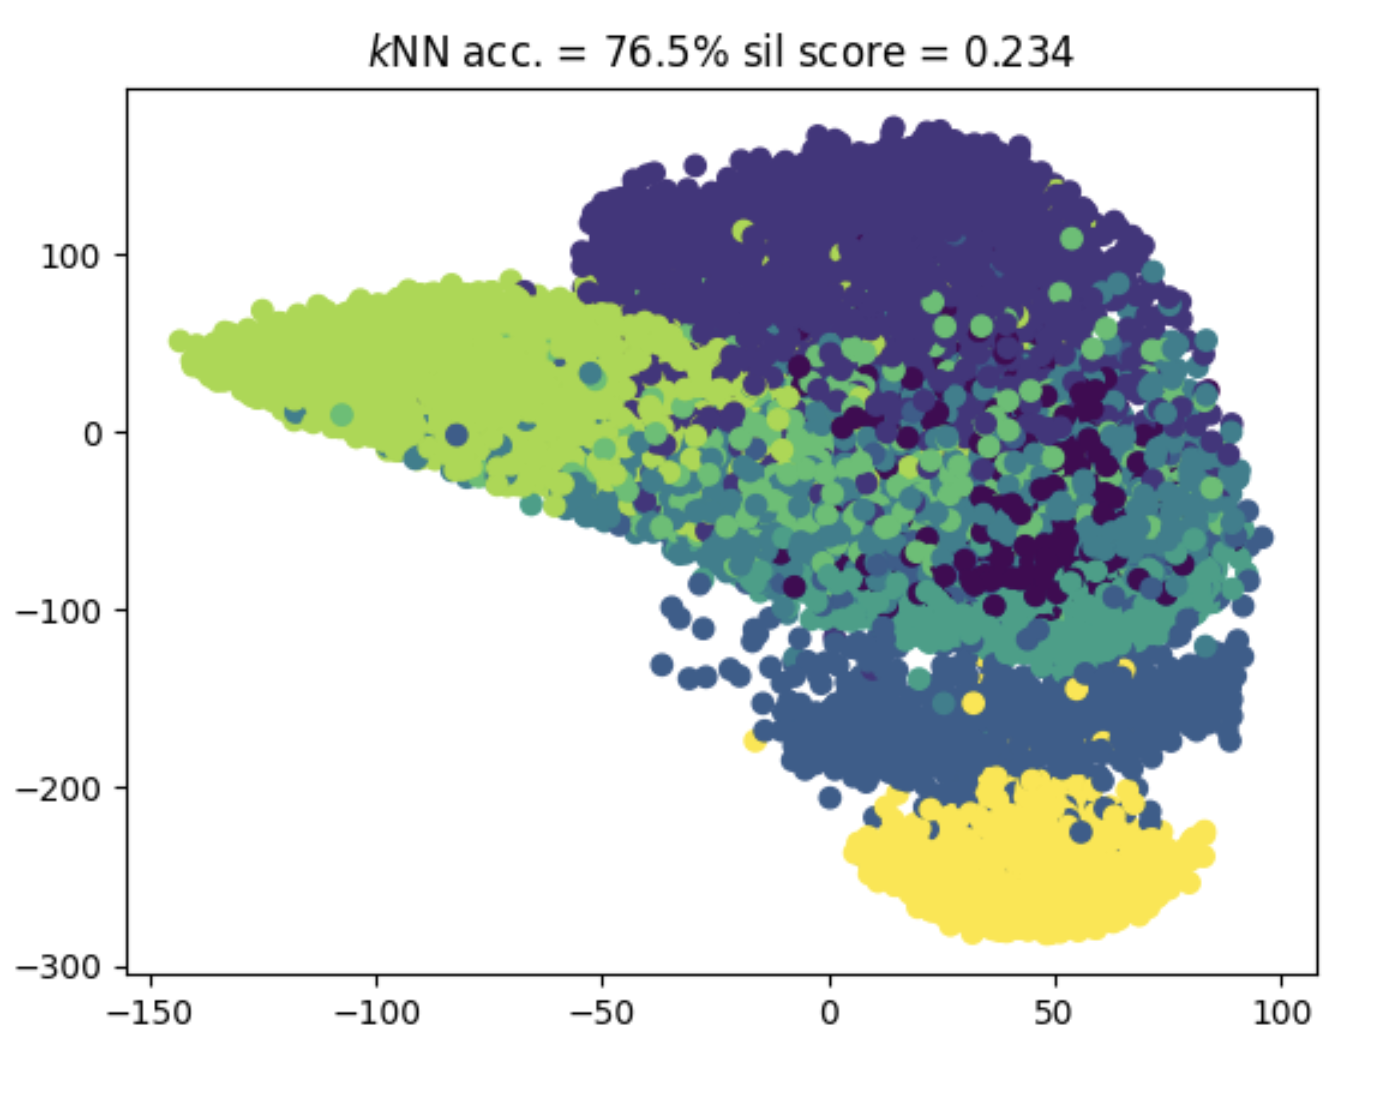
\includegraphics[width=\textwidth]{figs/cifar-10-tsimcne-2.png}
\caption{The visualization of the CIFAR-10 dataset using t-SimCNE with 150 epochs. Each color represents a separate class}
\label{fig:secex}
\end{figure}

\section{Hard Negative Sampling}
To amplify the contrastive learning signal by focusing on difficult yet informative negative examples, we integrated a hard negative sampling strategy into the existing InfoNCE loss function. The adapted InfoNCE loss, which we implemented as InfoNCECauchyHardNegative, has a temperature parameter and a beta parameter. The temperature controls the scale of the distribution, affecting the separation between similar and dissimilar points, while the beta parameter adjusts the emphasis on harder negatives.


\section{AUC-CL}

Besides the Hard Negative Sampling approach, we tested the loss function of the AUC-CL algorithm. It the same sense as previously, it calculates the similarity between features within each group and across the two groups using a similarity function that emphasizes features that are close in the feature space. This similarity function is fine-tuned with a temperature parameter, which helps control the sensitivity of the function to differences between features.

For the features that are similar, the loss function encourages the model to recognize and enhance these similarities, aiming to align similar features more closely. For the dissimilar feature pairs (those within the same group), the model is encouraged to distinguish between them more clearly. This is achieved by adjusting the emphasis on harder negative examples. This emphasis is controlled by another parameter in the loss function, which scales the impact of these harder negatives.

Furthermore, the function includes a dynamic adjustment mechanism, which regulates the contribution of each type of feature pair (similar and dissimilar) to the overall loss. This adjustment ensures that the model balances its attention between pulling similar items closer and pushing dissimilar items further apart in the feature space.

\section{Experimentation with Diverse Datasets}

To evaluate the efficacy and versatility of the modified loss functions, we conducted a series of experiments across multiple datasets. The primary objective was to assess how the modified t-SimCNE and t-SNE with SimCLR, as well as standalone t-SNE, perform in terms of the quality of visualization and the ability to capture meaningful class separations in different contexts. The datasets chosen for this study were CIFAR-10, Leukemia, Bloodmnist, and Dermamnist, each offering unique challenges and characteristics.

\subsection{Visualization Techniques}
\begin{enumerate}
\item {Standalone t-SNE}: As a baseline, standalone t-SNE was used to visualize the datasets without the influence of contrastive learning.
For each dataset, we applied three different visualization techniques:
\item {t-SNE with SimCLR}: We also explored a hybrid approach where t-SNE is applied to embeddings generated by SimCLR.
\item {t-SimCNE}: Our primary focus was on the modified t-SimCNE, which incorporates the newly adapted loss functions.
\end{enumerate}

\subsection{Implementation Details}
We adapted to the computational constraints and specific challenges posed by each dataset. Given the varying complexity and size of the datasets, the number of training epochs, batch sizes, and specific parameters for each visualization technique were tuned accordingly.
